\documentclass[TeamE-eindrapport]{subfiles}

\begin{document}
	
	\chapter{Het model}
	
%	\section{Accuraatheid}
%	
%	Om de accuraatheid van ons model te optimaliseren en te analyseren, splitsen we onze data op in 3 delen, zijnde de trainingsdata, de validatiedata en de testdata.
%	Vaak wordt de volledige dataset gesplitst in volgende verhoudingen: 50\% trainingsdata, 25\% validatiedata, 25\% testdata. Nadat het model is getraind met de trainingsdata, zullen we de validatiedata gebruiken om de optimale metaparameters te bepalen (zie \ref{tekst:validatie}). Tot slot kunnen we ons model testen op de testdata om te analyseren hoe goed het effectief werkt.
	
	\section{Bias}
	
	In machine learning verwijst bias naar de systematische fout die door een model wordt geïntroduceerd wanneer het de onderliggende patronen in de trainingsgegevens consequent verkeerd weergeeft. Dit kan leiden tot onnauwkeurige voorspellingen en onbetrouwbare prestaties op nieuwe datasets, zoals de validatie- en testdatasets.
	
	Wanneer we bias bespreken in de context van classificatie, verwijzen we vaak naar de neiging van het model om bepaalde klassen boven andere te bevoordelen. Er zijn dan twee belangrijke soorten bias die we willen toelichten.
	
	\subsection{\textit{Algorithmic bias}}
	
	\textit{Algorithmic bias} doet zich voor wanneer het algoritme zelf is getraind op een manier die bepaalde uitkomsten of groepen bevoordeelt. Het wordt bepaald door de gegevens die worden gebruikt voor training, en de keuze van het type model.
	Als een classificatiemodel bijvoorbeeld wordt getraind op vertekende gegevens die overwegend één groep vertegenwoordigen, kan het model leren nauwkeuriger te zijn voor die groep, terwijl het slecht presteert voor andere groepen. 
	
	Als we ons SVM model bijvoorbeeld bijna uitsluitend trainen op gevallen waar de tumor kwaadaardig is, zal het hoogstwaarschijnlijk niet goed presteren voor nieuwe datapunten waar de tumor goedaardig is. Het model is namelijk niet getraind op tumoren van die aard en zal dus geen nauwkeurige predicties kunnen doen.

	\subsection{\textit{Sampling bias}}
	
	\textit{Sampling bias} treedt op wanneer de trainingsgegevens niet representatief zijn voor de populatie waarnaar ze willen generaliseren. Dit kan gebeuren als bepaalde groepen in de populatie onder- of oververtegenwoordigd zijn in het trainingspakket. Als we ons SVM model bijvoorbeeld enkel trainen op tumoren van vrouwelijke borstkankerpatiënten, is de kans dat het model slecht presteert voor een nieuwe dataset van mannelijke patiënten vrij groot.
	
	\section{Variantie}
	
	De variantie is de maat voor de gevoeligheid van het model. Het geeft inzicht over de flexibiliteit van een model, met name hoe nauwkeurig de voorspellingen zijn bij verschillende datasets.

	Bij een hoge variantie is het model sterk aangepast aan de trainingsdata. Dit betekent dat zelfs kleine veranderingen in de trainingsdata een grote invloed zullen hebben op het model, wat resulteert in een fenomeen genaamd \textit{overfitting}. In het geval van tumorclassificatie zou een hoge variantie betekenen dat het model zeer nauwkeurig kan voorspellen of een tumor goedaardig is bij de trainingsdata. Maar doordat het model te sterk is afgestemd op de trainingsdata, zal het moeite hebben met generaliseren en levert dit geen precieze voorspellingen 	op voor de andere datasets, met name de validatie- en testdatasets.

	Aan de andere kant kan een model ook een te lage variantie hebben. Dit betekent dan dat het model te veel generaliseert en weinig verandert indien de trainingsdata verandert. Een te lage variantie leidt echter tot \textit{underfitting}. Hierdoor levert het ook geen betrouwbare voorspellingen op. Toegepast op tumorclassificatie zal een te lage variantie leiden tot een te sterk gegeneraliseerd model, waarbij het model niet goed presteert op de 3 verschillende datasets.
	
	\section{Flexibiliteit van het model bepalen}
	
	Hoe bepalen we nu de ideale flexibiliteit van ons model? Met andere woorden: hoe voorkomen we zowel \textit{overfitting}, waarbij het model de trainingsdata te nauwgezet probeert te volgen, als \textit{underfitting}, waarbij er sprake is van overgeneralisatie?
	
	\label{tekst:validatie}
	
	\subsection{Metaparameters}
	
	\label{tekst:metaparameter}
	
	Machine learning modellen hebben over het algemeen een of meerdere \textit{metaparameters} die de flexibiliteit van het model beïnvloeden. Het model zal zich meer of minder aanpassen naar gelang de waarden van deze metaparameter(s). Zoals we later zullen zien in hoofdstuk \ref{tekst:svm}, is een zekere \(\lambda\) de metaparameter die bij Support Vector Machines van belang is. Deze parameter wordt voor SVM ook wel de \textit{regularisatieparameter} genoemd. Deze \(\lambda\) zal uiteindelijk de breedte van de marge - en dus de variabiliteit van het model - beïnvloeden (zie later). 
	
	\subsection{Cross-validation}
	
	\label{tekst:crossvalidation}

	Om de optimale metaparameters te bepalen, gebruiken we het principe van \textit{cross-validation}. Hiervoor splitsen we eerst de data die we voor handen hebben op in 3 delen: 50\% trainingsdata, 25\% validatiedata, 25\% testdata. 
	
	De eerste stap is het trainen van ons model op de trainingsdata met een bepaalde waarde voor de metaparameter(s). Hierna zullen we de accuraatheid van dit model voor die bepaalde metaparameter(s) testen op de validatiedataset. Dit proces herhalen we voor - liefst zo veel mogelijk - verschillende waardes van de metaparameter(s), tot we de grootste accuraatheid van de voorspelling voor de trainingsdata hebben verkregen. De metaparameter(s) die voor de grootste accuraatheid zorgen op de trainingsdata, zullen we dan beschouwen als 'optimaal'. 
	
	We kunnen de accuraatheid van het getrainde model t.o.v. de trainingsdata uitzetten in functie van een metaparameter in een grafiek, zoals te zien is in figuur \ref{fig:metaparameter}. De waarde van de metaparameter waarvoor de grafiek die de accuraatheid weergeeft een maximum bereikt, zal de optimale waarde voor deze metaparameter zijn.
	
	\begin{figure}
		\centering
		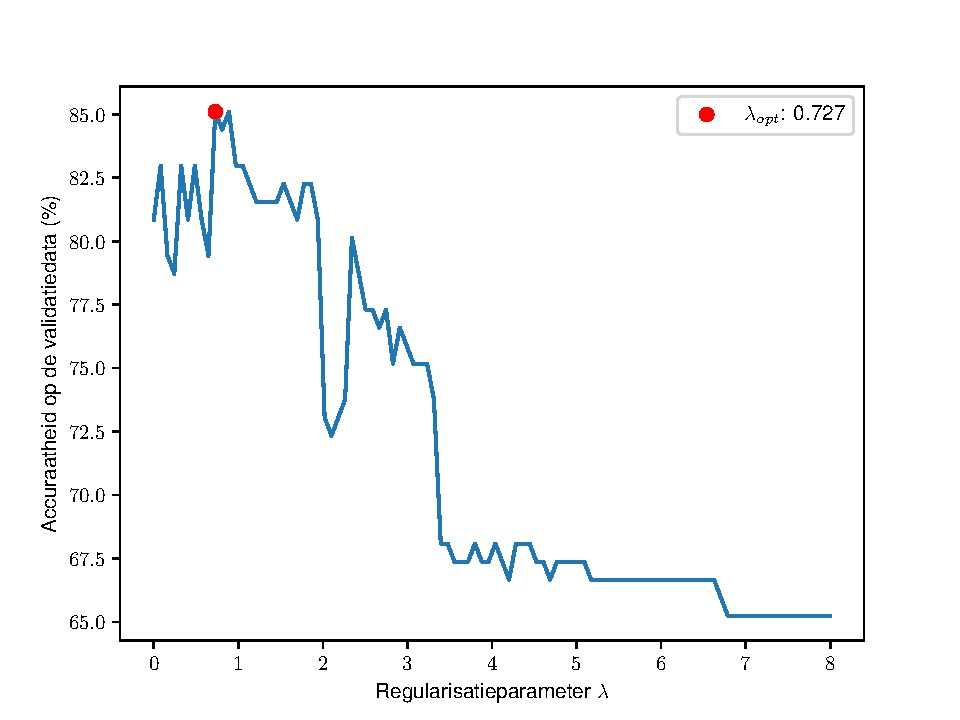
\includegraphics{accuraatheid}
		\caption{De accuraatheid van het model t.o.v. de trainingsdata, uitgezet in functie van de metaparameter \(\lambda\) voor ons SVM-model.}
		\label{fig:metaparameter}
	\end{figure}
	
	Tot slot gebruiken we onze testset om de algemene prestatie van ons model te beoordelen. Het uiteindelijke doel is om een zo goed mogelijke voorspelling te kunnen maken, gegeven een nieuwe set tumoren. We willen dus op basis van de 30 kenmerken de aard van nog niet eerder geziene tumoren voorspellen.
		
	%\begin{figure} deze afbeelding is niet zo relevant, want is van regressie
	%		\centering
	%		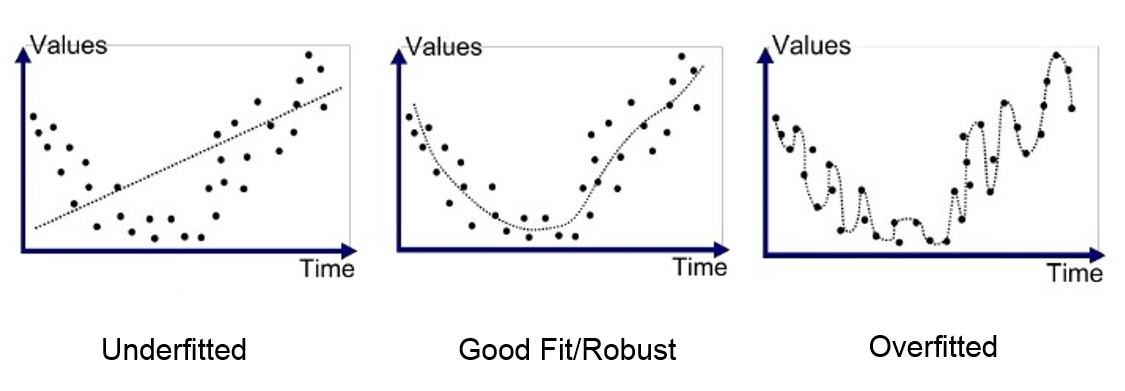
\includegraphics[width=\textwidth]{fitting}
	%		\caption{Illustratie van een underfitting, goeie fit en overfitting. Het eerste  model is duidelijk geen goed model omdat het niet aansluit bij de datapunten. het laatste model zal bij deze dataset een zeer goed model zijn, maar ook enkel voor dit model. Het is niet algemeen genoeg om op nieuwe data toe te passen. We proberen dus het middelste model te vinden die goed bij de punten aansluit maar niet te flexibel is. Afbeeldig: \textit{Nautiyal, Dewang} \cite{Nautiyal_2023}}
	%		\label{fig:fitting}
	%	\end{figure}

	
\end{document}